% Exemplo de relatório técnico do IC
% Criado por P.J.de Rezende antes do Alvorecer da História.
% Modificado em 97-06-15 e 01-02-26 por J.Stolfi.
% Last edited on 2003-06-07 21:12:18 by stolfi

% modificado em 1o. de outubro de 2008
\documentclass[11pt,twoside]{article}
\usepackage{techrep-ic}

%%% SE USAR INGLÊS, TROQUE AS ATIVAÇÕES DOS DOIS COMANDOS A SEGUIR:
\usepackage[brazil]{babel}
%% \usepackage[english]{babel}

%%% SE USAR CODIFICAÇÃO LATIN1, TROQUE AS ATIVAÇÕES DOS DOIS COMANDOS A
%%% SEGUIR:
%% \usepackage[latin1]{inputenc}
\usepackage[utf8]{inputenc}
\usepackage[dvips]{graphicx}
\usepackage{url}
\usepackage{multirow}
\usepackage{amsmath}

\bibliographystyle{abbrv}

\begin{document}

%%% PÁGINA DE CAPA %%%%%%%%%%%%%%%%%%%%%%%%%%%%%%%%%%%%%%%%%%%%%%%
% 
% Número do relatório
\TRNumber{???}

% DATA DE PUBLICAÇÃO (PARA A CAPA)
%
\TRYear{12}  % Dois dígitos apenas
\TRMonth{09} % Numérico, 01-12

% LISTA DE AUTORES PARA CAPA (sem afiliações).
\TRAuthor{R. Barboza Jr \and D. C. S. Lucas \and A. S. Ferreira}

% TÍTULO PARA A CAPA (use \\ para forçar quebras de linha).
\TRTitle{Uma Análise Comparativa Entre o Desempenho de Máquinas Virtuais Interpretadas de Sistema e de Processo}

\TRMakeCover

%%%%%%%%%%%%%%%%%%%%%%%%%%%%%%%%%%%%%%%%%%%%%%%%%%%%%%%%%%%%%%%%%%%%%%
% O que segue é apenas uma sugestão - sinta-se à vontade para
% usar seu formato predileto, desde que as margens tenham pelo
% menos 25mm nos quatro lados, e o tamanho do fonte seja pelo menos
% 11pt. Certifique-se também de que o título e lista de autores
% estão reproduzidos na íntegra na página 1, a primeira depois da
% página de capa.
%%%%%%%%%%%%%%%%%%%%%%%%%%%%%%%%%%%%%%%%%%%%%%%%%%%%%%%%%%%%%%%%%%%%%%

%%%%%%%%%%%%%%%%%%%%%%%%%%%%%%%%%%%%%%%%%%%%%%%%%%%%%%%%%%%%%%%%%%%%%%
% Nomes de autores ABREVIADOS e titulo ABREVIADO,
% para cabeçalhos em cada página.
%
\markboth{Barboza, Lucas e Ferreira}{Box}
\pagestyle{myheadings}

%%%%%%%%%%%%%%%%%%%%%%%%%%%%%%%%%%%%%%%%%%%%%%%%%%%%%%%%%%%%%%%%%%%%%%
% TÍTULO e NOMES DOS AUTORES, completos, para a página 1.
% Use "\\" para quebrar linhas, "\and" para separar autores.
%
\title{Uma Análise Comparativa Entre o Desempenho de Máquinas Virtuais Interpretadas de Sistema e de Processo}

\author{
 Roberto Barboza Jr
   \thanks{RA: 035712, rbarboza@gmail.com} \and
 Divino C. S. Lucas
   \thanks{RA: 115121, divcesar@gmail.com} \and
 Anderson Soares Ferreira
   \thanks{RA: 974530, asferreira.ferreira@gmail.com}
}

\date{}

\maketitle

%%%%%%%%%%%%%%%%%%%%%%%%%%%%%%%%%%%%%%%%%%%%%%%%%%%%%%%%%%%%%%%%%%%%%%%%%%%%%%%%%

\begin{abstract} 
Máquinas Virtuais são ferramentas amplamente utilizadas para resolução de 
diversos problemas computacionais e podem ser categorizadas por diversos atributos, 
entre eles escopo de emulação (sistema ou processo) e técnica de emulação 
(interpretação ou tradução). Como forma de ampliar a compreensão do \emph{overhead} 
decorrente da emulação do sistema operacional e dispositivos de \emph{hardware} em uma
máquina virtual de sistema, este trabalho apresenta uma comparação de 
desempenho entre máquinas virtuais interpretadas de sistema e de processo.
Para tanto, conduzimos uma investigação utilizando duas máquinas virtuais distintas. 
A primeira delas, chamada \emph{Bochs}, é uma máquina virtual de sistema que 
emprega interpretação como técnica de emulação, a segunda é uma máquina virtual 
de processo chamada \emph{Box}, desenvolvido a partir da ferramenta anterior 
especificamente para esse estudo.
\end{abstract}






\section{Introdução}
Uma Máquina Virtual (MV) é uma plataforma versátil que pode ser empregada para resolver diversos problemas na área de computação. 
Uma MV pode ser vista como uma camada utilizada para prover a integração entre duas interfaces (possivelmente distintas). 
Esta camada pode ser implementada com emulação em software, virtualização em hardware ou uma composição das duas abordagens.
As interfaces podem ser tanto a \emph{Application Binary Interface} (ABI) em MVs de processo, quanto a \emph{Instruction Set Architecture} (ISA) em MVs de sistema.
Dessa forma, tais ferramentas ocupam uma posição estratégica que pode ser explorada de diversas formas:
\textit{cross-platform emulation} - permitindo que aplicações escritas para uma plataforma sejam executadas em outra; 
\textit{simulação} - simulação do comportamento do hardware durante a execução do programa; \textit{análise} - análise do
perfil de execução das aplicações; \textit{otimização} - aplicar otimizações no código da aplicação utilizando informações
obtidas durante a execução do código.  

Duas abordagens são frequentemente empregadas para implementar a emulação de código em uma máquina virtual: interpretação e tradução.
Uma MV que emprega interpretação utiliza funções para simular o comportamento de cada instrução da aplicação sendo emulada. 
O processo de tradução porém, emprega técnicas da área de compiladores para produzir um código binário nativo (possivelmente otimizado) equivalente àquele da aplicação sendo emulada.
É comum encontrarmos MVs que, visando maximizar o desempenho, empregam estas abordagens em conjunto.

Note que uma MV de sistema emula não apenas as instruções da arquitetura alvo, mas toda uma infraestrutura de hardware
necessária para executar um sistema operacional. Nisto estão inclusos dispositivos como placa de rede, hierarquia de memória,
placa gráfica e etc. Para tarefas como \textit{cross-platform emulation} e perfilamento da execução do código de uma aplicação
em específico, o uso de uma MV de sistema também agrega ao \textit{overhead} de emulação da aplicação o \textit{overhead} de emulação destes 
dispositivos e do sistema operacional. Portanto frequentemente nestes cenários uma máquina virtual de processo é preferível
em relação a uma MV de sistema.

Nesse texto apresentamos uma proposta de avaliação do \textit{overhead} de emulação do sistema operacional e dispositivos de hardware em uma máquina virtual de sistema interpretada em relação a uma máquina virtual de processo interpretada. 

Para tanto, propomos a transformação de uma máquina virtual de sistema em uma máquina virtual de processo. 
Além de uma melhor compreensão do \textit{overhead} de emulação em uma máquina virtual de sistema, este trabalho tem como resultado uma infraestrutura para a realização de experimentos voltados para a área de máquinas virtuais. 

Este texto está organizado da seguinte forma. Na Seção~\ref{sec:objetivos} apresentamos com certo nível de detalhamento nossos objetivos. 
Na Seção~\ref{sec:fundamentacao} apresentamos a fundamentação teórica para a realização do projeto. Na Seção~\ref{sec:bibliografia} apresentamos um levantamento bibliográfico da área de máquinas virtuais a nível de binários. 
A Seção~\ref{sec:infraestrutura} e a Seção~\ref{sec:metodologia} descrevem a infraestrutura e a metodologia proposta para a realização do projeto, respectivamente. 
Por fim a Seção~\ref{sec:conclusao} apresenta a conclusão do trabalho. 
  
  
\section{Objetivos} \label{sec:objetivos}
As diferentes implementações de MVs apresentam características que determinam seu desempenho e aplicabilidade.
Por exemplo, implementações que utilizam a técnica de interpretação como único recurso para emulação de código tem como principal característica a portabilidade de código, permitindo que sejam utilizadas em diferentes plataformas. 
Em contrapartida, apresentam desempenho inferior a implementações que utilizam tradução dinâmica de binários.

% Acho que falta uma conexao entre esses dois parágrafos
% remover o parágrafo anterior é uma opcao 

Neste contexto, são escassos os dados sobre os custos relativos de executar um \textit{benchmark} em uma máquina virtual de sistema e de processos. 
No entanto, visto que a primeira abordagem apresenta o \textit{overhead} de emular todos os subsistemas de um computador real e ainda executar um sistema operacional completo, enquanto que a máquina virtual de processos apenas emula o sistema operacional, espera-se que o \textit{overhead} de emulação seja consideravelmente menor no segundo caso.
Desta forma, o objetivo geral deste trabalho é apresentar uma comparação entre o desempenho destes dois tipos de máquinas virtuais.
Como forma de atingir este objetivo, os seguintes objetivos específicos serão desenvolvidos:

\begin{itemize}
 \item Implementação de uma máquina virtual interpretada de processos a partir do emulador de sistemas Bochs;
 \item Implementação de mecanismos de otimização da técnica de interpretação como forma de reduzir o \textit{overhead} de emulação;
 \item Aplicação sistemática de teste, medição e análise de desempenho de aplicações executando nos dois cenários.
\end{itemize} 







\section{Fundamentação Teórica} \label{sec:fundamentacao}

\subsection{Máquinas Virtuais}

Uma máquina virtual tem como finalidade implementar as interfaces de um sistema a partir de outro sistema.
Seguindo a taxonomia apresentada por Jim Smith e Nair em \cite{Smith2005}, podemos classificar uma máquina
virtual em de sistema ou de processo dependendo de qual o escopo de emulação é provido:

\begin{itemize}
	\item \textbf{Máquina Virtual de Sistema:} A interface emulada é a nível da \emph{Instruction Set Architecture}. A ISA de
	um computador é composta de duas partes: as instruções de computação de propósito geral (\textit{user-ISA}) e as instruções de 
	controle dos periféricos do sistema (\textit{system-ISA}). Uma máquina virtual de sistema deve, portanto, emular tanto os dispositivos
	de hardware como placas de rede e vídeo quanto as instruções que controlam tais dispositivos. Dessa forma, uma máquina
	virtual de sistema permite a execução de um sistema operacional completo de forma transparente para a aplicação sendo
	emulada. 

	\item \textbf{Máquina Virtual de Processo:} A interface emulada é a nível da \emph{Application Binary Interface}. A ABI  
	define diversos padrões, onde os principais são: um subconjunto da ISA que é visível aos programas de usuário (\textit{user-ISA}) e uma 
	interface para que programas possam se comunicar com o sistema operacional para utilizar os recursos disponíveis no mesmo. 
	Em sistemas operacionais \textit{Unix-like}, esta interface com o sistema operacional é feita através de \emph{system calls} (syscalls). 

	A ABI também define convenções para tipos de dados, \textit{endianness}, alinhamento, chamadas de funções (como devem ser passados 
	os argumentos e o retorno), e o formato utilizado para representar arquivos binários executáveis e bibliotecas dinâmicas.
	No Linux o formato utilizado para representar tais arquivos é o \emph{Executable and Linking Format} (ELF).
\end{itemize}







\subsection{Técnicas de Emulação} \label{emulacao}

Segundo \cite{Smith2005}, a emulação é um processo de implementação das funcionalidades e interfaces de 
um sistema em outro sistema com características diferentes. Por exemplo, para criar uma máquina virtual
que executa um sistema compilado para o x86 em uma arquitetura PowerPC será necessário emular
tanto a interface do x86 (instruções) quanto funcionalidades (ex: \emph{calling convention}) utilizando
instruções disponíveis na arquitetura PowerPC. O processo de emulação é central em uma máquina virtual
e a técnica utilizada para implementá-lo é fundamental para o desempenho do sistema. Entre as técnicas 
frequentemente utilizadas para implementar emulação em uma máquina virtual estão: 

\begin{itemize}
  \item \textbf{Interpretação:} Processo no qual cada instrução do programa original (\emph{guest}) possui 
  uma rotina na plataforma destino (\emph{host}) que implementa a semântica da instrução na arquitetura \emph{guest}. 
  A interpretação envolve a recuperação da instrução original (\emph{fetch}), sua decodificação (\emph{decode}) 
  e finalmente a execução da operação equivalente.
 
  \item \textbf{Tradução de binários:} Neste processo um código nativo na arquitetura destino é gerado 
  dinamicamente (\emph{Just-in-time}) a partir do código original da aplicação e tem como função reproduzir o 
  comportamento do código da aplicação original \cite{Sites1993}. Esta forma de implementação assemelha-se ao
  processo de compilação estático onde um código fonte é decodificado e traduzido para uma linguagem destino.
 
  \item \textbf{Tradução em duas etapas:} Nesta forma de implementação, o sistema utiliza uma combinação de interpretação e tradução com o intuito de
  reduzir o \textit{overhead} de emulação. Regiões de código que são raramente executadas são apenas interpretadas
  (uma vez que o custo de tradução seria maior que o de sempre interpretar a região), enquanto porções de código que são 
  frequentemente executadas são traduzidas, uma vez que a execução do código de forma otimizada amortiza o custo da
  tradução.
\end{itemize}

As implicações do uso de interpretação ou tradução influenciam diretamente o desempenho e a aplicabilidade da 
máquina virtual. Em sistemas interpretados, o desempenho é relativamente baixo, uma vez que cada instrução é 
emulada individualmente por uma função, o que adiciona todo o \textit{overhead} de chamada e retorno de funções. Apesar 
disso, tais sistemas são extremamente portáveis, o que permite sua execução em diversas plataformas com poucas 
ou até mesmo nenhuma alteração em seu código original. Nos sistemas de traduções de binários, existe um custo 
(\emph{overhead}) inicial elevado, visto que o código original precisa ser traduzido antes de sua execução. 
No entanto, uma vez traduzido, o código resultante é executado nativamente, o que garante melhor desempenho. Sistemas
que empregam tradução em duas (ou mais) etapas são ainda mais sofisticados e utilizam técnicas para prever 
regiões de código que serão frequentemente executadas a fim de traduzir e otimizar tais regiões.

\subsection{Técnicas de Otimização para Interpretação}

Na forma mais básica de interpretação há um \textit{loop} principal que busca a instrução original, decodifica-a e chama 
a função responsável pela execução da instrução, retornando ao \textit{loop} principal logo em seguida. No entanto, 
existem diversas técnicas que tornam a interpretação um processo mais eficiente. Algumas delas estão listadas 
a seguir:

\begin{itemize}
 	\item \textbf{Threaded Interpretation:} São adicionadas ao final das funções que emulam cada uma das instruções a 
 	busca pela próxima instrução, sua decodificação e a chamada para a função responsável pela execução da instrução. 
 	Note que isto reduz drasticamente o número de iterações do \textit{loop} principal do interpretador.

 	\item \textbf{Pre Decoding:} As instruções são decodificadas, por exemplo, sempre que uma nova página de código é 
 	carregada do disco, e os campos como \emph{opcode} e operandos são salvos em estruturas de dados padronizadas, o 
 	que torna possível uma implementação mais simples e eficiente dos mecanismos de despacho e interpretação. 
 	
 	\item \textbf{Direct Threaded Interpretation:} Utilizado em conjunto ao \textit{Pre Decoding}. Anota-se junto com
 	as informações de decodificação o endereço da rotina que deve fazer a interpretação de cada instrução, de forma que
 	ao final de cada rotina de interpretação é feito um salto indireto ``diretamente'' para a rotina que interpreta a
 	próxima instrução - evitando a consulta por uma rotina de instrumentação.  

	\item \textbf{DICache:} É uma proposta de utilização de uma cache de decodificação para as instruções interpretadas
	frequentemente. A DICache \cite{dicache} funciona como uma cache convencional e pode ser implementada tanto em software como em 
	hardware. Cada linha da cache contém uma rótulo para identificar a instrução mapeada para aquela linha, os operandos
	da instrução e o endereço da rotina que faz a interpretação dessa instrução.
\end{itemize}

\subsection{Executable and Linking Format}

O \emph{Executable and Linking Format} (ELF) \cite{SCO1997} é o formato de arquivos binários executáveis, 
bibliotecas compartilhadas, códigos objetos, etc. utilizados em ambientes \textit{Unix-like}. Um arquivo ELF
encaixa-se em um dos três tipos:

\begin{itemize}
 	\item \textbf{Relocatable File:} Representa um arquivo objeto que contém dados e código que serão ``linkados" 
 	a outro binário para criar um executável ou objeto compartilhado. Em geral são arquivos utilizados durante
 	o processo de compilação estática.
 
 	\item \textbf{Executable File:} Representa um programa compilado. O programa pode possuir dependências que
 	devem ser resolvidas em tempo de execução ou pode ter ``linkagem" estática, o que significa que todas as bibliotecas
 	necessárias para sua execução já foram resolvidas durante a compilação.
 
 	\item \textbf{Shared Object:} Representa um biblioteca dinâmica que contém código e dados que podem ser 
 	``linkados" a outro objeto compartilhado, criando um terceiro objeto compartilhado, ou pode ser combinado a 
 	um executável pelo \textit{linker} dinâmico e a outros objetos compartilhados para a criação de uma imagem de processo.
\end{itemize}

A organização de um arquivo ELF é composta por um cabeçalho principal (\emph{ELF Header}), seguido por cabeçalhos 
de seção - descrevendo seções de informações (instruções, dados, símbolos) utilizados na ``linkagem" estática - ou cabeçalhos 
de programa - que contém os segmentos da aplicação e as informações necessárias para a criação do processo. 







\section{Levantamento Bibliográfico}  \label{sec:bibliografia}

O Bochs \cite{bochs} é uma máquina virtual de sistema com suporte a emulação 
de diversos processadores da família x86 32 e 64 bits. Ele preza por portabilidade, 
e nesse sentido utiliza interpretação como técnica de emulação. Para reduzir o 
\textit{overhead} de interpretação, o Bochs utiliza técnicas como \emph{pre-decoding}~\cite{Magnusson1994}, 
\emph{threaded-interpretation}~\cite{Klint1981}, e \emph{lazy evaluation}~\cite{Hookway1997}.
O sistema que estamos propondo se diferencia do Bochs por ser voltado à emulação 
de processos e não de sistemas.

O Pin \cite{Luk2005} é uma máquina virtual de processo que emula os ISAs IA-32 e 
x86-64. Ele é uma ferramenta de código fechado e possui versões tanto para Windows 
como para Linux, sendo reconhecido por prover uma rica API para criação de 
ferramentas (Pintools) para análise do comportamento dinâmico de aplicações. O Box 
difere do PIN por ser uma máquina virtual de código aberto e utilizar interpretação 
como técnica de emulação. Em contrapartida, estes dois sistemas tem em comum o 
aspecto de proverem uma interface para instrumentação de binários e serem emuladores 
\emph{same-ISA}~\footnote{Em uma máquina virtual same-ISA as duas interfaces da 
máquina virtual são iguais, possivelmente diferindo apenas em relação a ABI.}.

O HDTrans \cite{Sridhar2006} é uma máquina virtual de processo para a arquitetura 
IA-32. O HDTrans difere do Bochs e do PIN por empregar tradução de binários como 
técnica de emulação. No entanto, o HDTrans abre mão de empregar otimizações no 
código traduzido (o que geralmente é feito para amortizar o \textit{overhead} de tradução) 
em favor da implementação de uma tradução simples e rápida. O Box diferencia-se do 
HDTrans por empregar interpretação de binários.

O Dynamo \cite{Bala2000} é uma máquina virtual de processo para a arquitetura do 
HP PA-8000. Diferentemente do PIN, Bochs e HDTrans, o Dynamo é uma máquina virtual 
cujo objetivo é otimizar a execução do programa sendo emulado. Para tanto, o Dynamo 
emprega uma combinação das técnicas de interpretação e emulação. O sistema 
inicialmente interpreta o código da aplicação sendo emulada. Uma vez que uma região 
é declarada como quente~\footnote{Uma região de código é quente quando ela é 
frequentemente executada.}, o Dynamo aplica otimizações nesta região e salva o 
código otimizado em uma cache de traduções. Subsequentes invocações do trecho de 
código original serão emuladas utilizando o código traduzido. O Box diferencia-se 
do Dynamo por não ter o foco na otimização de binários mas sim em ser um sistema 
que disponibilize uma interface simples para instrumentação de binários.

O IA-32 EL \cite{Baraz2003} é uma máquina virtual de processos com o objetivo de 
suportar a execução de aplicações IA-32 em processadores da família IA-64. De forma 
similar ao Dynamo, o IA-32 EL emprega uma abordagem de emulação em duas etapas, 
porém as duas etapas realizam tradução de código. Inicialmente o IA-32 EL efetua a 
tradução de código em uma granularidade de bloco básico. Durante essa tradução, 
código de instrumentação é inserido para detectar blocos básicos quentes. Quando um 
número mínimo de blocos básicos é identificado, o sistema forma uma região de código 
envolvendo esses blocos básicos, os otimiza e posteriormente salva em uma cache de 
traduções. Execuções subsequentes desses blocos básicos usam a tradução otimizada. 
O Box diferencia-se do IA-32 EL por não fazer tradução de binários.

O StarDBT \cite{Wang2007} é uma máquina virtual de pesquisa capaz de fazer traduções de 
aplicações compiladas para x86 32/64 bits para execução em hardware x86 32 bits. De 
forma similar ao IA-32 EL e ao Dynamo, o StarDBT é um tradutor em duas fases. Regiões 
de código que são infrequentemente executadas são traduzidas utilizando um tradutor 
simples e rápido, enquanto regiões de código que são frequentemente executadas são 
traduzidas empregando otimizações de código e posteriormente persistidas em uma cache 
de traduções. O Box diferencia-se do StarDBT por ser capaz de traduzir apenas binários 
de 32 bits, compilados para Linux e não empregar tradução de binários.

% Acho que seria interessante colocarmos alguns papers que investigaram sobre
% o overhead de emulação em máquinas virtuais, especificamente sobre a emulação
% de sistemas operacionais em relação a processos. Será que achamos? Será que tem? 




\section{Infraestrutura de Pesquisa} \label{sec:infraestrutura}

Como citado na Seção~\ref{sec:objetivos}, o projeto proposto utilizará como
ponto de partida para o desenvolvimento o emulador de sistema Bochs. Portanto 
a infraestrutura inicial em termos de código fonte será a já presente no Bochs. 
O código fonte do Bochs é escrito em linguagem C++ e disponibilizado para download
no Sourceforge \cite{bochs_site}. Para iniciar o desenvolvimento do Box, criaremos
um \emph{branch} do código fonte do Bochs no sistema de versionamento distribuído
GitHub \cite{github}, isto permitirá que os membros do projeto desenvolvam o sistema
de forma colaborativa.

O \textit{benchmark} utilizado para fazer o teste e a análise de desempenho dos sistemas será
o MiBench~\cite{Guthaus2001}. Este \textit{benchmark} foi escolhido por ser gratuito, possuir
um número razoável de programas (mais de 35) representativos de diversos cenários de 
aplicação, serem programas com uma pequena base de código e terem um curto período
de execução.

Nenhum hardware, software ou material de consulta além daqueles já adquiridos 
pelos membros do projeto será necessário para o desenvolvimento do projeto.





\section{Metodologia}  \label{sec:metodologia}

Como forma de atingir o objetivo proposto, o trabalho adotará uma abordagem 
dividida em três etapas logicamente divididas em passos, que serão descritos 
em detalhes a seguir.

\subsection{Implementação da máquina virtual de processos}

Nesta etapa será implementada a versão básica da máquina virtual. O 
interpretador proposto utilizará a infraestrutura da interpretador Bochs 
como ponto de partida para desenvolvimento. Por ser uma máquina virtual de 
sistema, o Bochs implementa mecanismos de emulação para diversos subsistemas 
de hardware, como BIOS, hierarquia de memória, placas de vídeo e de rede, etc. 
Tais subsistemas são desnecessários em uma máquina virtual de processos, visto 
que esses dispositivos não são acessíveis diretamente por programas de usuário, 
e por esse motivo serão removidos do projeto.

\begin{figure}[h]
 \centering
 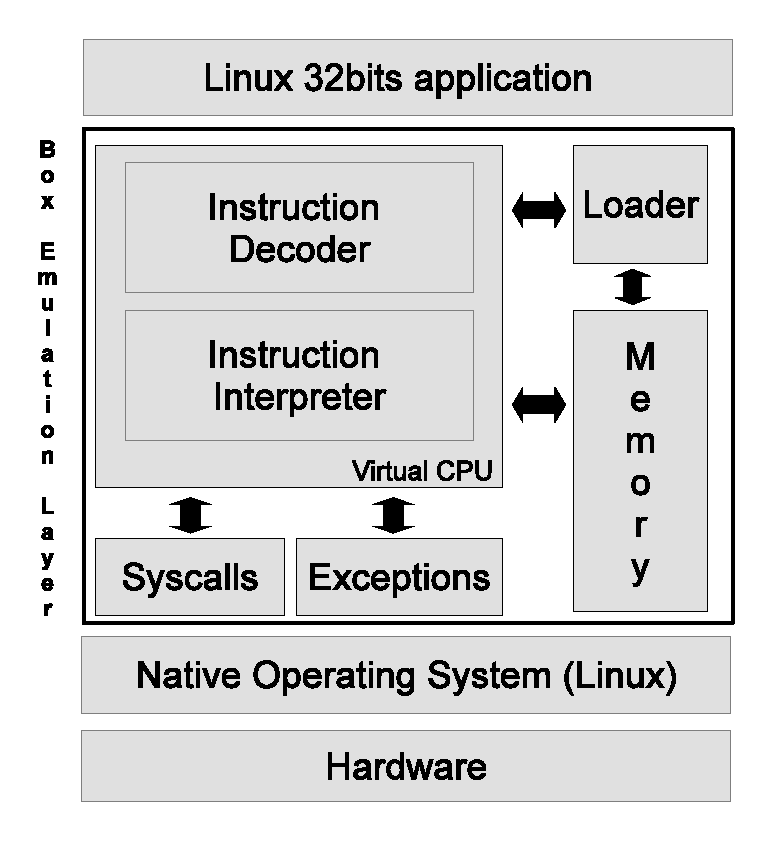
\includegraphics[width=0.5\columnwidth]{./figures/box-architecture.eps}
 \caption{Arquitetura do interpretador de processos Box. 
 O Box é uma máquina virtual same-ISA para aplicações compiladas para Linux x86 32 Bits.}
 \label{fig:box-architecture}
\end{figure}

A Figura \ref{fig:box-architecture} apresenta a arquitetura geral do interpretador.
O sistema será composto de seis módulos principais que serão gerenciados pelo \textit{runtime}
da máquina virtual: carregador, emulador de memória, decodificador, interpretador, 
emulador de chamadas de sistema e emulador de exceções. Utilizando esta arquitetura 
será possível carregar e interpretar um executável Linux de 32 Bits com ligação dinâmica. 
Segue abaixo a descrição de cada um destes módulos:

\begin{itemize}
    \item \textbf{Carregador:} É o módulo responsável por ler, decodificar e resolver as
    dependências dinâmicas do executável principal e bibliotecas compartilhadas. A entrada 
    desse módulo é o binário principal a ser emulado e a saída é o espaço de endereçamento 
    onde a interpretação do processo ocorrerá.

    \item \textbf{CPU:} Este módulo é composto por dois componentes principais: o decodificador
    e o interpretador. A CPU é responsável por controlar o fluxo de emulação da aplicação.
    Nesse sentido ela direciona o decodificador a buscar e decodificar uma instrução no
    módulo de memória para em seguida passar a informação decodificada para o módulo de 
    interpretação, que emulará o comportamento da instrução decodificada.

    \item \textbf{Memória:} Módulo responsável pelo gerenciamento do espaço de memória reservado 
    para a aplicação, suas dependências, área de \textit{stack} e \textit{heap}. Este módulo é o responsável por
    emular leituras e escritas na área de dados do espaço de endereçamento.

    \item \textbf{Chamadas de sistema:} Este módulo é composto por rotinas que são \textit{wrappers}
    para as \emph{system calls} do sistema nativo. Quando o processo sendo emulado faz uma
    syscall, o interpretador decodifica a interrupção e redireciona a execução para a rotina
    que simula o comportamento da \textit{system call} desejada. 
    
    \item \textbf{Exceções:} Este módulo é o responsável pelo gerenciamento de exceções 
    geradas pele programa sendo emulado e redirecioná-las para os devidos tratadores de
    exceção, ou encerrar a execução do programa. 
\end{itemize}

\subsection{Otimização da máquina virtual}

Nesta etapa serão implementados os passos que adicionarão ao interpretador 
recursos de instrumentação e otimização de desempenho da interpretação.

\begin{itemize}
    \item \textbf{Otimização:} Neste passo implementaremos uma das seguintes 
    técnicas: DICache~\cite{Chen2012} ou Threaded-Interpretation~\cite{Klint1981}.
    Como descrito na Seção~\ref{sec:fundamentacao} essas técnicas tem o objetivo 
    de agilizar o processo de busca e despacho das instruções a serem interpretadas.
 
    \item \textbf{Instrumentação:} Neste passo implementaremos suporte para 
    instrumentação dinâmica das aplicações emuladas. Recursos como interceptação
    de acessos a memória, detecção de instruções de desvio e interrupções serão 
    adicionados ao sistema base.
\end{itemize}
 
\subsection{Análise de desempenho}

Nesta etapa serão conduzidos testes e medições para analisar o desempenho do sistema
proposto em relação ao emulador Bochs. Essa etapa é divida em duas partes:

\begin{itemize}
    \item \textbf{Análise 1:} Nesta análise avaliaremos o desempenho da versão 
    base do sistema proposto em relação ao emulador de sistema Bochs. Para 
    isto, utilizaremos uma versão do Box que não consta com otimizações além 
    daquelas já implementadas no Bochs. O resultado deste passo será a quantificação
    do \textit{overhead} decorrente da emulação do sistema operacional e dispositivos de
    hardware em uma máquina virtual de sistema. 
    
    \item \textbf{Análise 2:} Nesta análise iremos avaliar o impacto das técnicas 
    de otimização implementadas na etapa 2 no desempenho do sistema. O resultado
    deste passo será a quantificação do \textit{speedup} (ou \textit{overhead}) decorrente da 
    utilização de tais técnicas.
\end{itemize}

Como descrito anteriormente na Seção~\ref{sec:infraestrutura}, o \textit{benchmark} 
MiBench~\cite{Guthaus2001} será utilizado para fazer a análise do sistema
proposto.







\subsection{Cronograma}

A Tabela~\ref{tab:cronograma} apresenta o cronograma previsto para o desenvolvimento do Box.
Cada linha representa uma das etapas/passos descritos nas subseções anteriores. Cada coluna representa
uma semana durante o desenvolvimento, a primeira semana inicia-se no dia 25 de setembro e a
última semana encerra no dia 21 de novembro, totalizando 8 semanas.

\begin{table}[h]
\centering
\begin{tabular}{|l|c|c|c|c|c|c|c|c|} \hline
\multicolumn{1}{|c|}{\multirow{2}{*}{\textbf{Atividade}}} & \multicolumn{8}{c|}{\textbf{Semana}} \\ \cline{2-9}
\multicolumn{1}{|c|}{} & 1\textsuperscript{a} & 2\textsuperscript{a} & 3\textsuperscript{a} & 4\textsuperscript{a} & 5\textsuperscript{a} & 6\textsuperscript{a} & 7\textsuperscript{a} & 8\textsuperscript{a} \\ \hline
CPU             & $\bullet$ & $\bullet$ &  &  &  &  &  &  \\ \hline
Carregador  	& $\bullet$ & $\bullet$ & $\bullet$ &  &  &  &  &  \\ \hline
Memória     	& $\bullet$ & $\bullet$ & &  &  &  &  &  \\ \hline
Syscalls    	&  & $\bullet$ & $\bullet$ &  &  &  &  &  \\ \hline
Exceções    	&  & $\bullet$ & $\bullet$ &  &  &  &  &  \\ \hline
Otimizações 	&  &  &  & $\bullet$ & $\bullet$ & $\bullet$ &  &  \\ \hline
Análises    	&  &  &  &  & $\bullet$ & $\bullet$ & $\bullet$ &  \\ \hline
Relatório Final	&  &  &  &  &  &  & $\bullet$ & $\bullet$ \\ \hline
\end{tabular}
\caption{Cronograma de desenvolvimento do Box}
\label{tab:cronograma}
\end{table}

Este projeto será desenvolvido por três alunos, portanto justificando a sobreposição
de tarefas no cronograma. Além disso note que alguns desses componentes já faziam 
parte da base de código do Bochs (por exemplo: decodificador e interpretador) e
outros (como syscalls, memória e carregador) já tiveram seu desenvolvimento iniciado
antes da escrita deste relatório.






\section{Conclusão}  \label{sec:conclusao}

Este trabalho apresentou uma proposta de análise de desempenho entre máquinas 
virtuais interpretadas de sistema e de processo.

Além dos dados provenientes desta análise, o trabalho também apresenta como 
contribuição o desenvolvimento de uma máquina virtual interpretada de processos para 
aplicações Linux x86 de 32 Bits. Embora o desenvolvimento desta ferramenta esteja 
voltado para a produção de dados para a análise de desempenho, tal ferramenta 
pode ser utilizada em situações como instrumentação e simulação de aplicações 
e como módulo de compatibilidade para execução de aplicações \textit{Unix-like} x86 
32 Bits em diferentes sistemas operacionais ou arquiteturas.

A implementação e análise de técnicas de otimização de desempenho para 
interpretadores fornecerá resultados que poderão ser aplicados em outros 
emuladores para melhorar ou compreender melhor o desempenho do sistema. 





\bibliography{box}




\end{document}
